\documentclass[a4paper,german,12pt,smallheadings]{scrartcl}
\usepackage[T1]{fontenc}
\usepackage[utf8]{inputenc}
\usepackage{babel}
\usepackage{tikz}
\usepackage{geometry}
\usepackage{amsmath}
\usepackage{amssymb}
\usepackage{float}
\usepackage[thinspace,thinqspace,squaren,textstyle]{SIunits}
\restylefloat{table}
\geometry{a4paper, top=15mm, left=20mm, right=40mm, bottom=20mm, headsep=10mm, footskip=12mm}
\linespread{1.5}
\setlength\parindent{0pt}
\begin{document}
\begin{center}
\bfseries % Fettdruck einschalten
\sffamily % Serifenlose Schrift
\vspace{-40pt}
Analytische Mechanik, Sommersemester 2013, 4. Blatt \\
Luis Herrmann und Markus Fenske, Tutor: Clemens Meyer zu Rheda
\vspace{-10pt}
\end{center}
\section*{Aufgabe 1}

Wir gehen hier von einer Rotation um die x-Achse aus, während in der
Aufgabenstellung eine Rotation um die y-Achse gegeben ist. Die Probleme sind
äquivalent. Wir ermitteln zuerst die minimale Funktion für eine Rotation um die
x-Achse und bilden dann die Umkehrfunktion.

%\resizebox{10cm}{10cm}{%
\begin{figure}[H]
  \begin{center}
    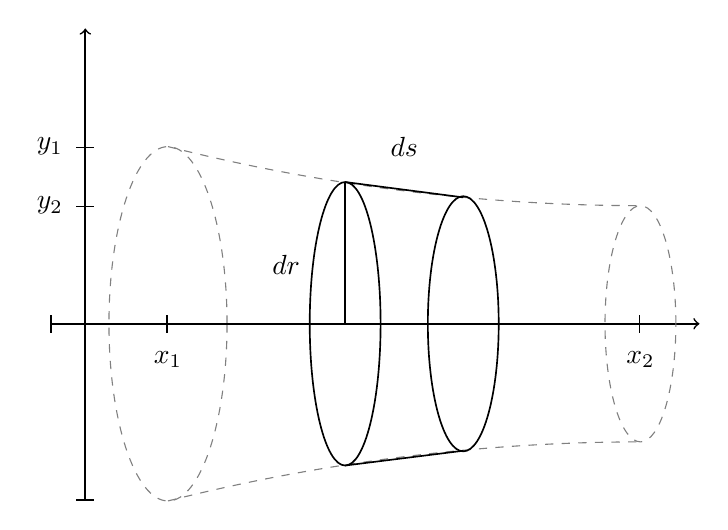
\begin{tikzpicture}[scale=1.5]
      \draw[dashed,color=gray] (0,1.5) ellipse (0.5 and 1.5);% right half of the left ellipse
      \draw[dashed,color=gray] (0,0) parabola bend (4,0.5) (4,0.5);% bottom line
      \draw[dashed,color=gray] (0,3) parabola bend (4,2.5) (4,2.5);% top line
      \draw[semithick] (1.5,1.5) ellipse (0.3 and 1.2);% left du
      \draw[-,semithick] (1.5,2.7) -- (2.5,2.57);
      \draw[-,semithick] (1.5,1.5) -- (1.5,2.7); % dr
      \draw (1.0,2) node {$dr$};
      \draw (2.0,3) node {$ds$};
      \draw[semithick] (2.5,1.5) ellipse (0.3 and 1.08);% left du
      \draw[-,semithick] (1.5,0.3) -- (2.5,0.425); % bottom ds
      \draw[|-|,semithick] (-1,1.5) -- (0,1.5);
      \draw[-|,semithick] (0,1.5) -- (4,1.5);
      \draw[->,semithick] (4,1.5) -- (4.5,1.5);
      \draw[|-|,semithick] (-0.7,0) -- (-0.7,2.5);
      \draw[-|,semithick] (-0.7,2.5) -- (-0.7,3);
      \draw[->,semithick] (-0.7,3) -- (-0.7,4);
      \draw (-1,2.5) node {$y_2$};
      \draw (-1,3) node {$y_1$};
      \draw[dashed,color=gray] (4,1.5) ellipse (0.3 and 1);% right ellipse
      \draw (0,1.2) node {$x_1$};
      \draw (4,1.2) node {$x_2$};
    \end{tikzpicture}
  \end{center}
  \caption{Rotationskörper mit Radiuselement $dr$ und Linienelement $ds$}
\end{figure}
%}

Der Abbildung kann man den Aufbau des Integrals entnehmen. Die Gesamtfläche des
Rotationskörpers ist zusammengesetzt aus einzelnen zylinderförmigen
Teilelementen $dA$. Die Mantelfläche dieses Zylinders berechnet sich durch $dA
= 2\pi dr \cdot ds$. Dabei ist $dr$ der Radius und $ds$ die Breite des
Zylinders (siehe Grafik). \textbf{Notiz:} Grafik nochmal überarbeiten. Die
Fläche $dA$ soll eine Zylinderoberfläche sein, kein Kegelstumpf. Scheiß
Infinitesimalkalkül!

Der Radius entspricht der Höhe der zu ermittelnden Funktion an der
entsprechenden Stelle, also $dr = 2 \pi f(x)$. Die Breite ergibt sich durch das
Kurvenlängenelement $ds = \sqrt{dx^2 + dy^2} = \sqrt{1 +
\left(\frac{dx}{dy}\right)^2} dx$

Insgesamt ist unser zu minimierendes Integral dann also:

\begin{equation}
  I[f] = \int_{x_1}^{x_2} 2 \pi f(x) \sqrt{1 + f'(x)^2}\; dx
\end{equation}

Das Problem lösen wir mithilfe der Euler-Lagrange-Gleichung. Sei $L = f
\sqrt{1+f'^2}$. Dann muss die minimierende Funktion die Lösung folgenden
Gleichung sein:

\begin{align*}
  &\frac{d}{dt} \frac{\partial L}{\partial f'} = \frac{\partial L}{\partial f} \\
  \Leftrightarrow &\frac{d}{dt} \frac{ff'}{\sqrt{1 + f'^2}} = \sqrt{1 + f'^2} \\
  \Leftrightarrow &\frac{ff'' + f'^4 + f'^2}{(1+f'^2)^\frac{3}{2}} = \sqrt{1 + f'^2} \\
  \Leftrightarrow &ff'' + f'^4 + f'^2 = (1 + f'^2)^2 \\
  \Leftrightarrow &ff'' + f'^4 + f'^2 = 1 + 2f'^2+f'^4 \\
  \Leftrightarrow &ff'' + f'^2 = 1 + 2f'^2 \\
  \Leftrightarrow &ff'' - f'^2 = 1
\end{align*}



\end{document}
